\chapter{System Implementation} \label{ch:implementation}
\section{Overview of Network Functions} \label{sec:desc_nfv_overview}

While \cite{che-wei-master} focused on the design of vCPE platform, this paper focused on the design of VNF itself. Our network functions (Fig. \ref{fig:nfv_overview}) are designed with SDN-enabled NFV architecture concept \cite{sdn-enabled}, using the synergies between computer infrastructures (NFVs) and network infrastructures (NFVIs) \cite{etsi-nfv-terminology, etsi-nfv-infra}. An NFV is a VNF controller, mainly used for addressing stateful processing and NFVI is an SDN switch used for stateless processing.


\subsection{Stateful Processing Component}
This component is used to control the workflow, maintain the state associated with the VNF, and provide an interface for service providers or customers to configure and update the behavior of the stateless datapath processing component. We used an SDN controller to implement the VNF controller; and notably, we use southbound APIs of the SDN controller framework to manage the interface between the stateful and stateless components with the OpenFlow protocol, which was originally designed for this purpose.


\subsection{Stateless Processing Component}
Stateless processing component is implemented by SDN datapath resources and is optimized for data plane traffic processing. Because an SDN switch can be decoupled with control plane and data plane, the switch can accept the control messages from the stateful processing component.

By using the advantages of this architecture, we can assign stateless or light-weight state work to the SDN switch (e.g., packet filtering and packet counting) to reduce the load on the computing resources. If we want to update our service, we are required to update only the stateful component, because the stateless component merely follows the commands from the stateful component.

\begin{figure}[!t]
\centering
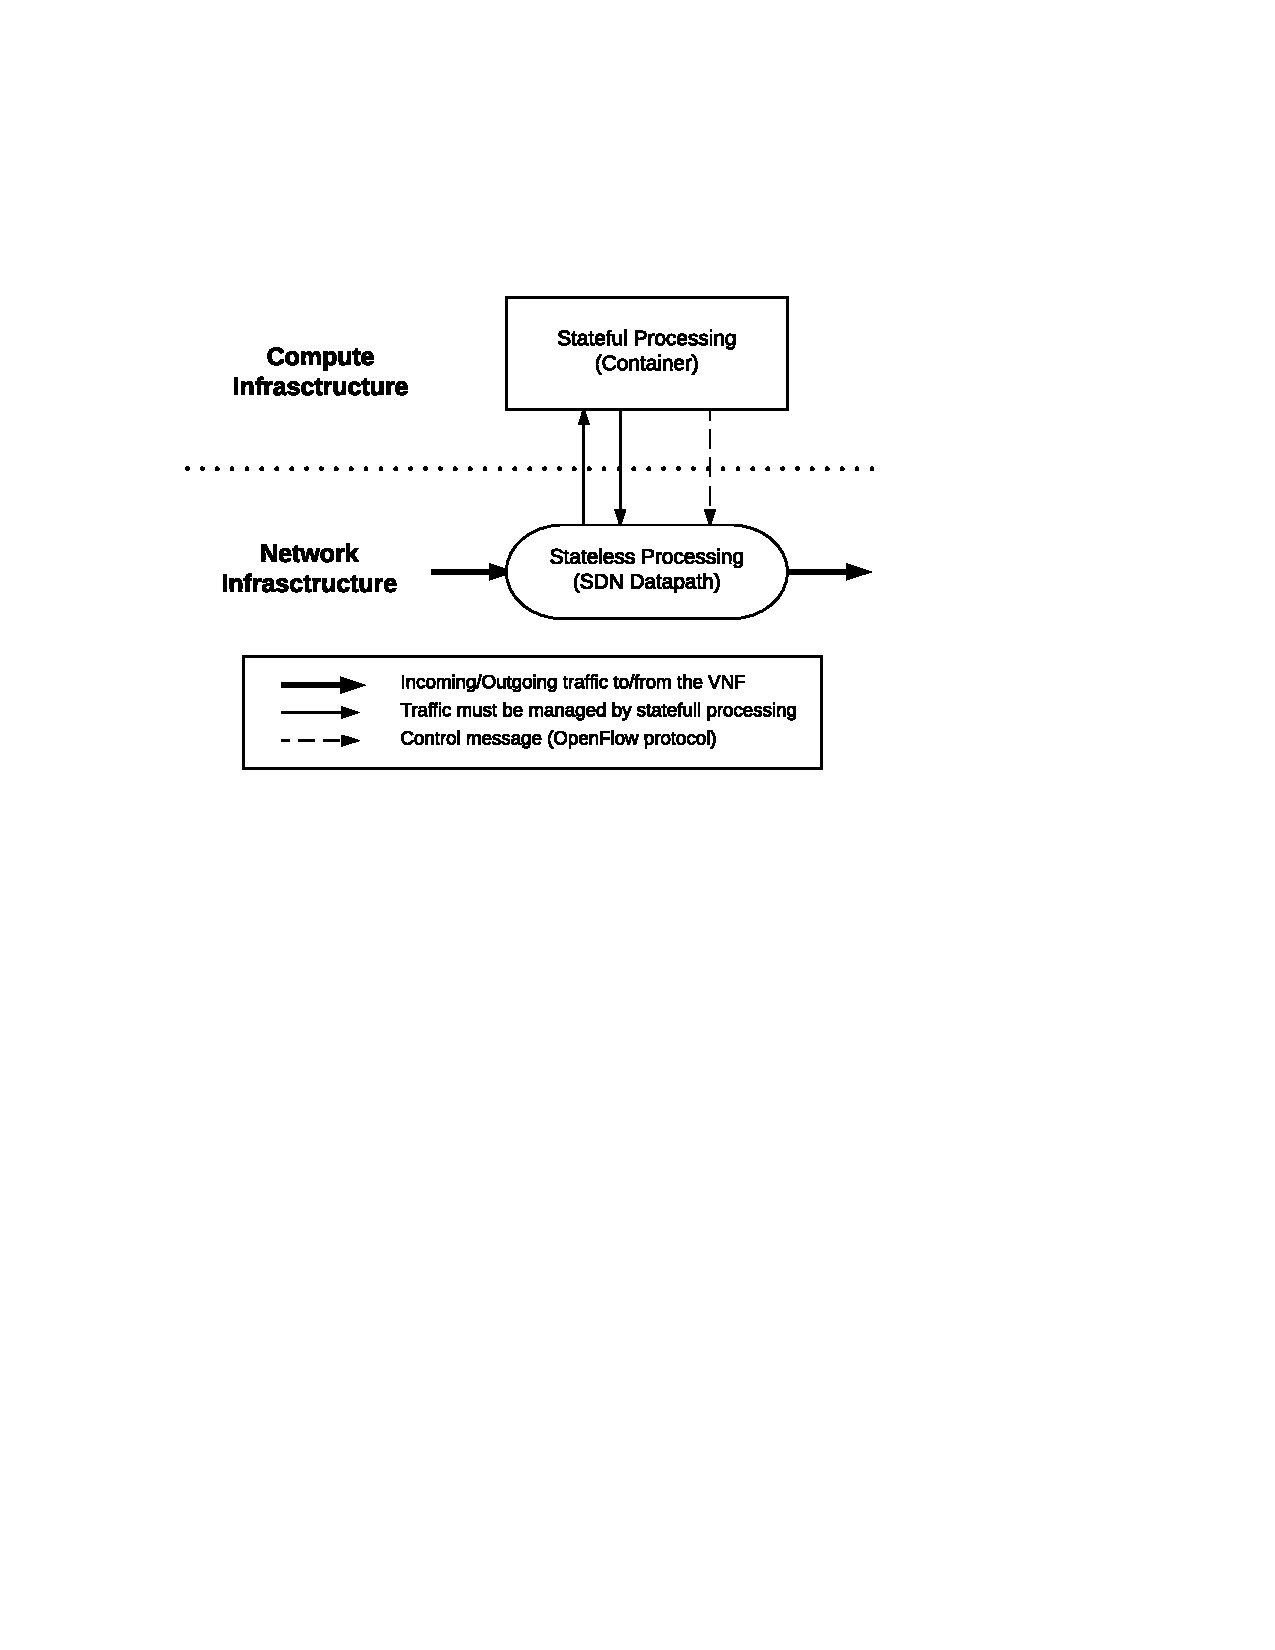
\includegraphics[width=0.8\textwidth]{./fig/nfv_overview.pdf}
\caption{Overview of network functions.}
\label{fig:nfv_overview}
\end{figure}

\begin{figure*}[!t]
\centering
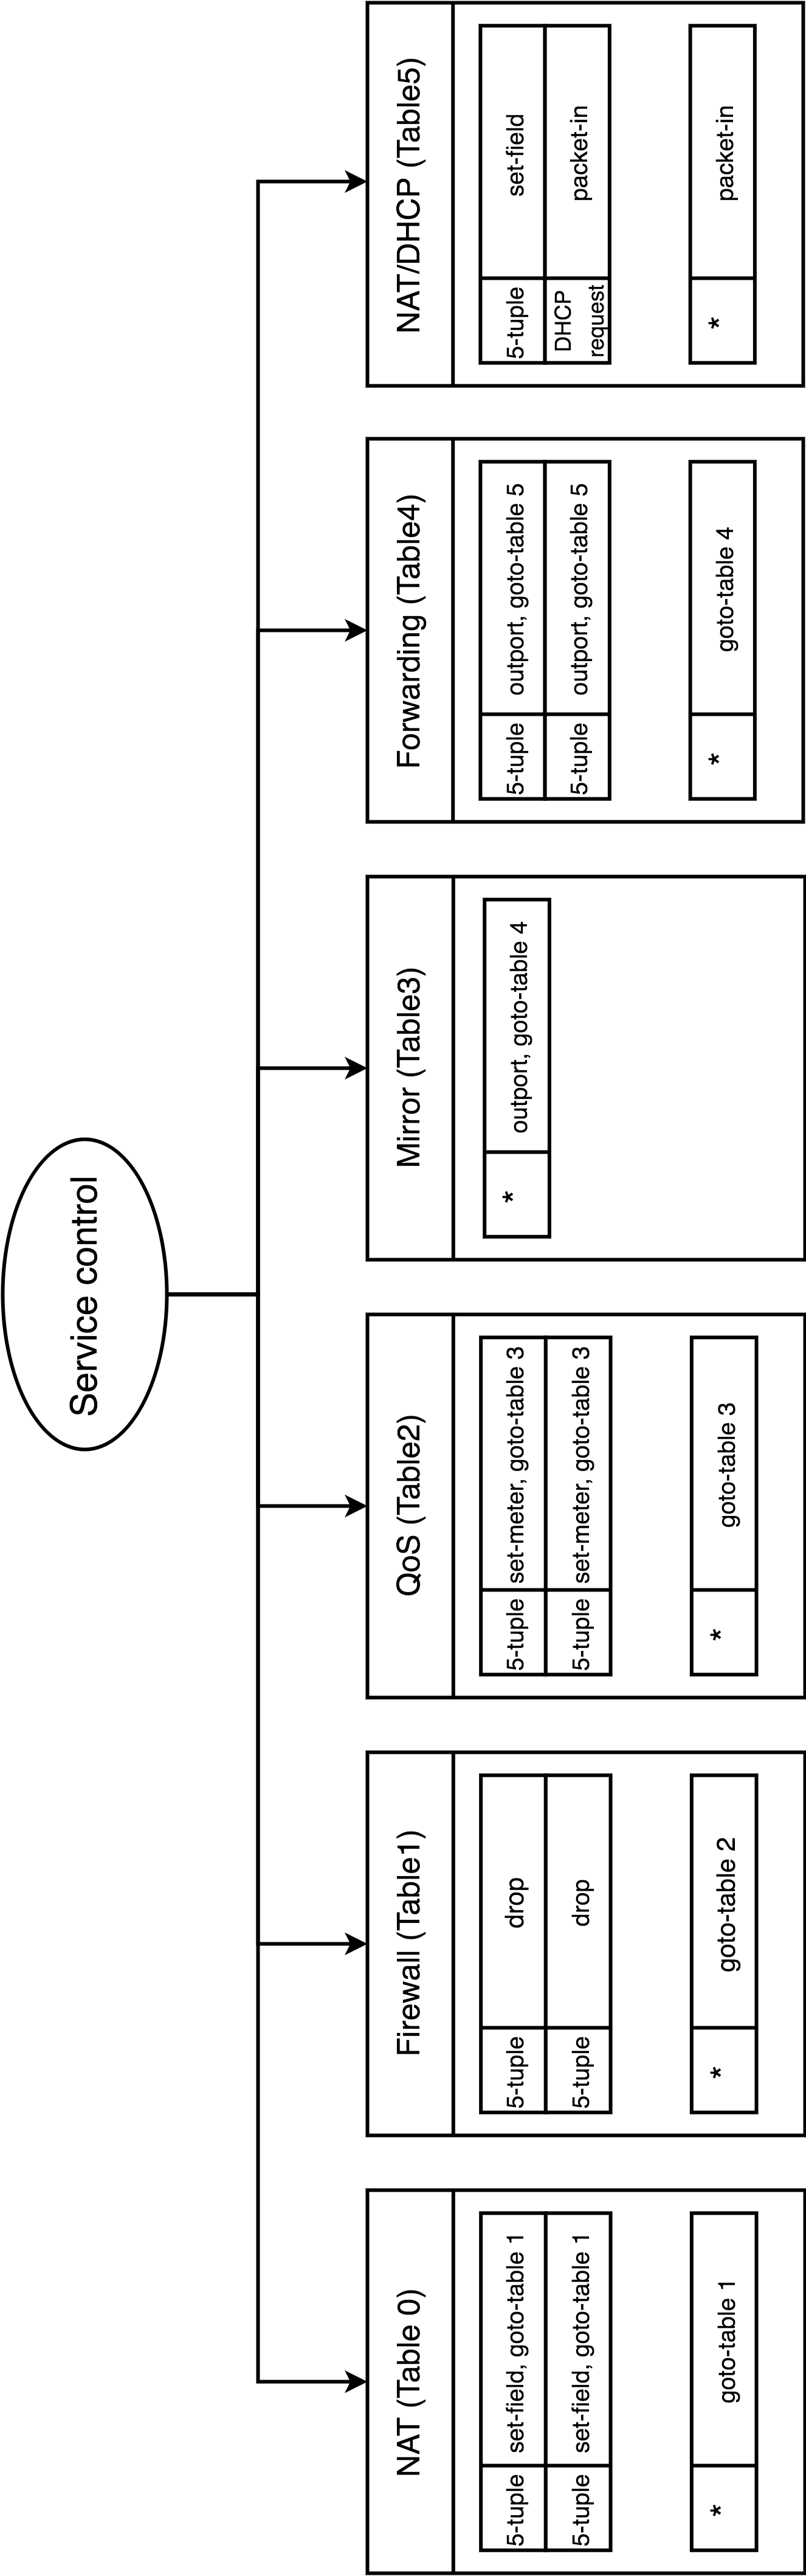
\includegraphics[width=\textwidth]{./fig/mft_table_overview}
\caption{Flow table order of vCPE service.}
\label{fig:mft_table_overview}
\end{figure*}



\section{Multiple Flow Table Strategy} \label{sec:multi_flow_table_strategy}
In section \ref{sec:desc_nfv_overview}, we introduce the vCPE service design architecture. The network functions are managed through cooperation between the SDN controller on the cloud and SDN switch at the local network gateway. The controller transforms the network functions into a series of OpenFlow rule requests and sends it to the SDN switch. Following the orders from the controller, the SDN switch inserts the rules into its flow tables, examines the incoming packets against the flow entry match fields, and executes the actions in matching rules. The flow table \cite{sdn-ft} defines all matching and corresponding processing, thus playing an important role in the executive network function.

We found that a single flow table restricts the implementation of our network functions. In \cite{multiple-flow-table}, two conditions under which a single flow table is too restrictive were reported. The first is a condition where a single packet must perform independent actions based on matching with different fields. The second is a condition where the packet requires two-stage processing. To satisfy both conditions, we implemented the network functions by using a multiple flow table strategy.

Before we discuss about the multiple flow table strategy, we introduce the pipeline of OpenFlow flow table first \cite{openflow-spec}. The processing of each packet always starts at the first flow table. When being processed by a flow table, the packet is matched the flow entries of the flow table and adds corresponding action to the instruction set. The packet can executes the instrcution set immediately, or execute after finishing the journey in switch. A flow entry can direct a packet to next table by go-to action. In our multiple flow table management model, we set the ``go to next table'' action as the table-miss action. Therefore, the packet is processed table-by-table in a certain sequence.

In a multiple flow table strategy, it is most important to determine which flow table the rules should be inserted into. We used the network function as a demarcation, that is, SDN applications responsible for specific network functions inserted rules into one specific flow table to enable us to focus on the design of the network function itself. However, the order of the flow table and the sequence of the network functions become crucial. This can be addressed by considering the type of match and action in the rules generated by the network function.

The network functions of vCPE services are the firewall service, NAT, DHCP, forwarding, and QoS. The order of each function was determined as shown in Fig. \ref{fig:mft_table_overview} (note that the flow tables are counted from zero). Each packet In the following sections, we introduce the method of implementing these network functions, the type of rules to be inserted into the SDN switch, and the effect of these rules on deciding the order of the flow tables.



\section{Service Control} \label{sec:service_control}
Service control is used to enable or disable services. To enable a service, the table-miss rule should be modified. A packet-in rule is always placed in the flow table of the last active service as a table miss in case there is no corresponding rule. To enable the service chain, the rules of each service except the last service contain an additional action, ``go to next flow table'', which enables the packets to continue to pass through all active services.

To disable a service, we must not only modify the table-miss rule but also add an enforce rule. Each enforce rule has maximum priority with the action, ``go to next flow table''. It indicates that packets still pass through the disabled service’s table, but ignore other rules and proceed to the next flow table.



\section{Network functions} \label{sec:setwork_functions}
\subsection{Firewall}
The firewall service can dynamically block traffic and prevent the packets from causing a packet-in event.
On the dashboard, we can specify the blocking policies. There are three kinds of policies:
\begin{enumerate}[leftmargin=4em]
  \item block any traffic from a source IP or destination IP address;
  \item block traffic based on known layer 4 protocols, such as SSH and HTTP;
  \item block traffic to customize layer 4 ports of a host.
\end{enumerate}

For different policies, the controller applies corresponding rules to the SDN switch. After the policies are set, the blocking rules are immediately installed. Subsequently, any traffic that satisfies the blocking criteria is dropped. Normal traffic is unaffected.

As shown in Table \ref{table:fw}, all the actions of flow entries are dropped. The first rule illustrates that SSH connection with the source IP address 192.168.2.1 is blocked. The second rule indicates that the flow entry blocks the Telnet protocol.

In our multiple flow table model, the firewall service is located in flow table 1 because once packets are detected by the blocking rules, they do not need to be applied to any other services. The packets that satisfy the blocking rules are immediately dropped, and their journey in the flow table ends. The other unblocked packets pass all blocking rules and finally satisfy the table-miss rule, which allows the packets to proceed to the next flow table. The action of the firewall is different from those of other services, because in other services, irrespective of the actions taken with the packets, the packets must proceed to the next flow table.

% firewall example table
\begin{table*}[!t]
\caption{Firewall rules in Flow Entry}
\label{table:fw}
\centering
\begin{threeparttable}
\begin{tabular}{|l|l|l|l|l|l|}
\hline
IP proto & IP src      & IP dst       & L4 sport & L4 dport & action \\ \hline
TCP      & 192.168.2.1 & *            & *        & 22       & drop   \\ \hline
TCP      & *           & *            & *        & 23       & drop   \\ \hline
\end{tabular}
  \begin{tablenotes}
    \item[] Symbol * represents wildcard (matches any value).
  \end{tablenotes}
\end{threeparttable}
\end{table*}


\subsection{NAT}
The NAT service allows numerous hosts to use one public IP address for connecting to the network. To achieve this, the SDN controller must set the packet header field. Because the SDN switch sets the field, the first packet must proceed to the controller. When the controller adds the flow to the SDN switch, the packet does not proceed to the controller. This can reduce the burden on the controller.

Following is an example that illustrates the modification of the IP address and port number by using the NAT service. For an outgoing packet, the SDN switch does not have any flow entry in the flow table, and hence, a packet-in event is triggered initially. The packet that is sent by a private network host is sent to the SDN controller, and the packet header fields are modified using the set-field action. The source IP address and source port number of the outgoing packet are modified to a public IP address and a new port number is remapped for NAT. For the incoming packet, the destination IP address and destination port number are modified to fit the private IP address and port number. Subsequently, the SDN controller adds these flow entries to the SDN switch; all packets must be sent to the controller

In Fig. \ref{fig:mft_nat}, the public IP address of NAT is 140.114.71.178, and the host private IP address is 192.168.8.254 with the port number 7878. The client sent the packet to a server with the IP address 140.114.71.177 and port number 9898.

As shown in Table \ref{table:nat}, when the host sends the packet to the server (outgoing), a packet-in event is triggered, and the packet is sent to the controller. The set-field action modifies the source IP address to a public IP address of NAT, 140.114.71.178, and the source port to 2000. When the server sends the packet back to the client (incoming), the packet header field is modified. The destination IP address and destination port number are modified to 192.168.8.254 and 7788, respectively.

In the single flow table framework, two rules must be added to the SDN switch to match the outgoing and incoming situations. First, we predicted that the NAT service must be placed in the last table of the multiple flow table framework because the NAT service must set the packet header fields and enable connection to the outside network. Most importantly, the SDN switch is placed according to the order of tables to match the field. The outgoing and incoming situations must be considered. In consideration of all the aforementioned factors, we place the NAT service in the first and last tables in our multiple flow table framework.

\begin{figure}[!t]
\centering
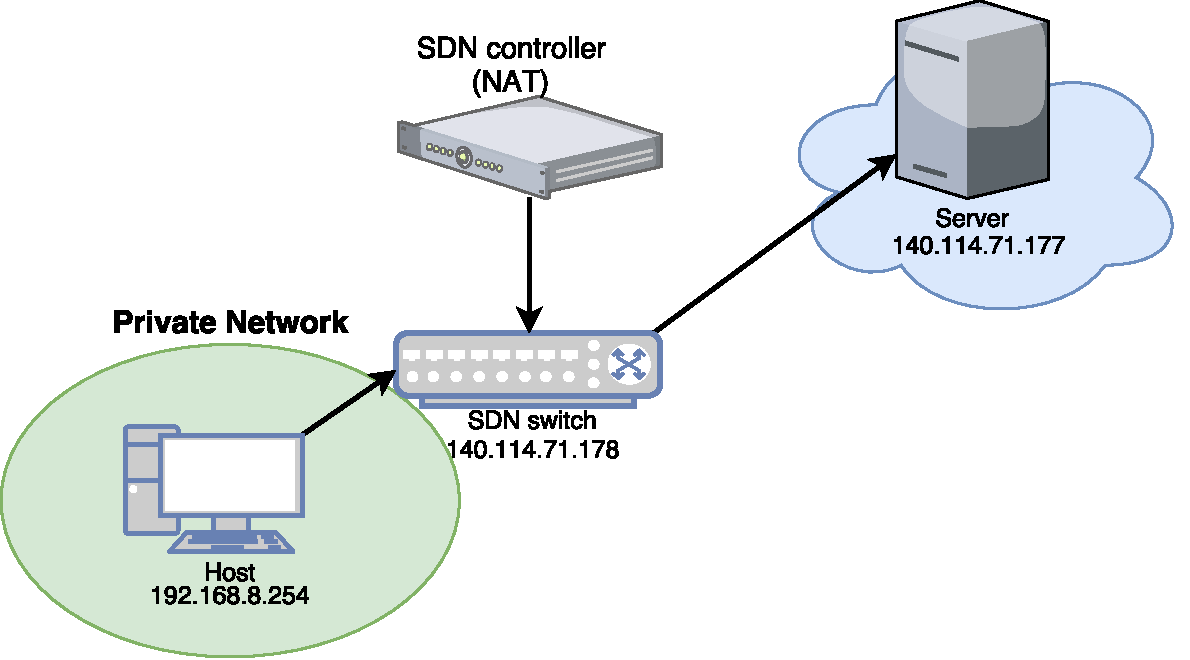
\includegraphics[width=0.8\textwidth]{./fig/mft_nat.pdf}
\caption{Example of modification of IP address and port number by NAT service.}
\label{fig:mft_nat}
\end{figure}

% NAT example table
\begin{table*}[!t]
\caption{Flow entry for modifying the packet header fields}
\label{table:nat}
\centering
\begin{tabular}{|l|l|l|l|l|l|}
\hline
Direction & IP src         & IP dst          & src port     & dst port    &  action  \\ \hline
Outgoing  &192.168.8.254   &140.114.71.177   & 7878         & 9898        & \begin{tabular}[c]{@{}l@{}}IP src $\,\to\,$ 140.114.71.178; \\ L4 src port $\,\to\,$ 2000\end{tabular} \\ \hline
Ingoing   &140.114.71.177  &140.114.71.178   & 9898         & 2000        & \begin{tabular}[c]{@{}l@{}}IP dst $\,\to\,$ 192.168.8.254; \\ L4 dst port $\,\to\,$ 7878\end{tabular} \\ \hline
\end{tabular}
\end{table*}


\subsection{DHCP}
The DHCP service implements the DHCP protocol to dynamically assign IP addresses to hosts. A DHCP operation uses the UDP protocol. Clients use port 68 as the source port and port 67 as the destination port. By contrast, the server uses port 67 as the source port and port 68 as the destination port. Our system can handle packets to realize the DHCP service.

This service is executed through the following steps:
\begin{enumerate}
\item The controller adds a DHCP rule for DHCP packets when the service is enabled.
\item All packets match this DHCP rule, causing a packet-in event.
\item The controller determines whether a packet is a DHCP discovery packet. If so, the controller assigns an IP address, generates a DHCP offer, and then performs a packet-out event. If not, the controller determines whether it is a DHCP request. If the result is positive, the controller generates a DHCP acknowledgement and then performs a packet-out event.
\end{enumerate}

Our system supports multiple flow tables; however, a specific flow table for the DHCP service is not required because only one rule is installed for all hosts who request the DHCP service. When the service is disabled, the DHCP rule is deleted, and the packets continue to pass through our service chain. The subsequent DHCP packets can reach other DHCP servers by forwarding service.


\subsection{Forwarding} \label{ssec:forwarding}
In the forwarding service, when the first packet in a new connection is incoming, a packet-in event occurs because no corresponding rule is present. When the controller receives the packet, it records the IP-layer information, including the source IP address, destination IP address, input port number, source MAC address, and destination MAC address. By using the recorded information, the controller can install a 5-tuple forwarding rule with out-port action for this connection, and the subsequent packets do not need to undergo the packet-in event. The 5-tuple comprises the source IP address, destination IP address, network layer protocol, source layer 4 port, and destination layer 4 port.

To gather per-session statistical information, 5-tuple rules are required. Therefore, rules based on the MAC address are not added. The controller installs a pair of dummy rules for every connection, and then requests the switch to obtain current flow statistics every second. Thus, the real-time bandwidth statistics of each connection can be obtained by merely subtracting the byte count from the byte count of the last second.


\subsection{QoS}
QoS is mainly used for traffic control. Two management functions are provided for QoS. We first introduce three strategies and then discuss the flow table order of QoS in the multiple table model.

\subsubsection{Rate Limitation of Hosts}
When some hosts utilize a high network bandwidth, the speed for other hosts slows or traffic congestion occurs. To prevent these effects, rate limiting is used to control the rate of traffic from a host. For implementing the host rate limitation, we first create a meter for the desired bandwidth and then add a flow, of which the match is the host’s MAC address and the action is the meter.

This method is illustrated in \ref{fig:mft_qos_rate_host}. In T0, host 1 and host 2 are not limited yet. Because host 2 utilizes a substantial amount of bandwidth from the network in T0–T1  the network administrator sets the host 2 rate limit to 400 Kbps. When the controller receives this request, marked as (a), it creates a meter with meter id = 1 and bandwidth = 400 Kbps and sets the rule in the flow table with the destination MAC address = MAC address of host 1 and meter = 1. According to our new flow table, it limits the rate of the target host. Then, the traffic from host 2 is reduced and immediately limited to 400 Kbps. A similar situation occurs for host 1 in T2. The administrator chooses to set host 1 under 600 Kbps, marked as (b), and then the traffic from host 1 is limited to 600 Kbps.

\begin{figure}[!t]
\centering
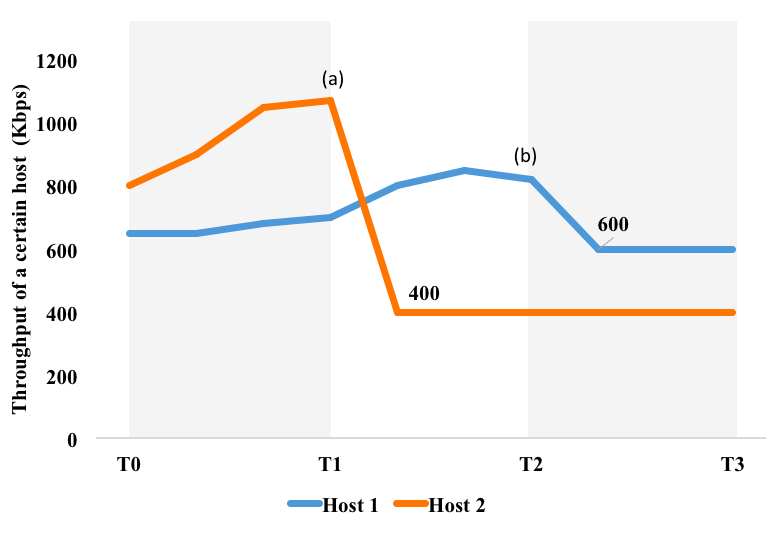
\includegraphics[width=0.8\textwidth]{./fig/mft_qos_rate_host}
\caption{Illustration of rate limiting for a certain host}
\label{fig:mft_qos_rate_host}
\end{figure}

\subsubsection{Rate Limitation of Applications}
An increasing number of network applications such as online games, video streaming, and conference calls are used. Therefore, substantial traffic exists in the network. Consequently, we integrated a flow classification engine to identify which application the flow belongs to. The integration scenario is presented in Fig. \ref{fig:class_classifying}.

To rate the limit for a certain application, we must first gather per-flow statistical information. When a connection is created, the first packet of the connection is handled by the forwarding service and the 5-tuple rules are added into the SDN switch to obtain the bandwidth information of the per-flow connection (see Section \ref{ssec:forwarding} for details). With the classified result of application identification, the application type of each connection can be determined.

When the network administrator requests to rate limit a certain application to a certain bandwidth, the bandwidth is equally distributed to each connection of the application. The controller sets all flows that belong to the same application into the same meter, and the bandwidth of the meter is modified to achieve the desired value. For example, suppose that we can determine which flows belong to an application through the flow classification engine. This application is to be limited to 1000 Kbps. In T0 (Fig. \ref{fig:mft_qos_rate_app}), three connections belong to this application, and the bandwidth of the meter to each link is set as 333 (1000/3) Kbps. In T2, two connections are added to this application, and the bandwidth of the meter to each link is reset as 200 (1000/5) Kbps. In T2, one connection is obtained in this application, and hence, the bandwidth of the meter to each link is reset as 250 (1000/4) Kbps. However, the sum of bandwidth from this application should always be 1000 Kbps. In other words, the bandwidth is dynamically adjusted.

It is worth noting that we did not change any rules in flow table; we merely change the bandwidth of the correspond meter in the meter table to reduce the overhead of switch and controller.

\begin{figure}[!t]
\centering
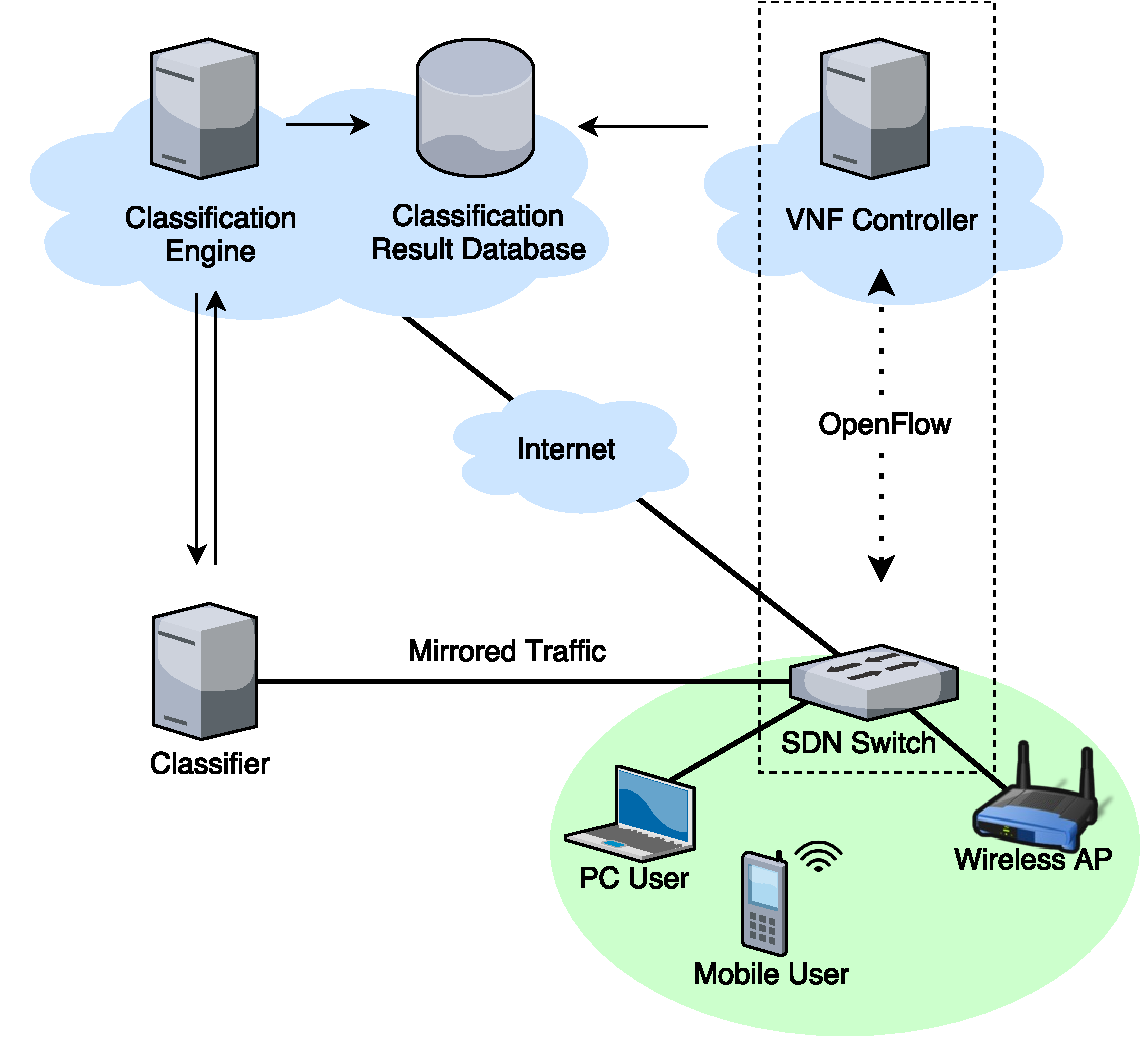
\includegraphics[width=0.8\textwidth]{./fig/classification_classifying}
\caption{Architecture of our application identification system in classification phase.}
\label{fig:class_classifying}
\end{figure}

\begin{figure}[!t]
\centering
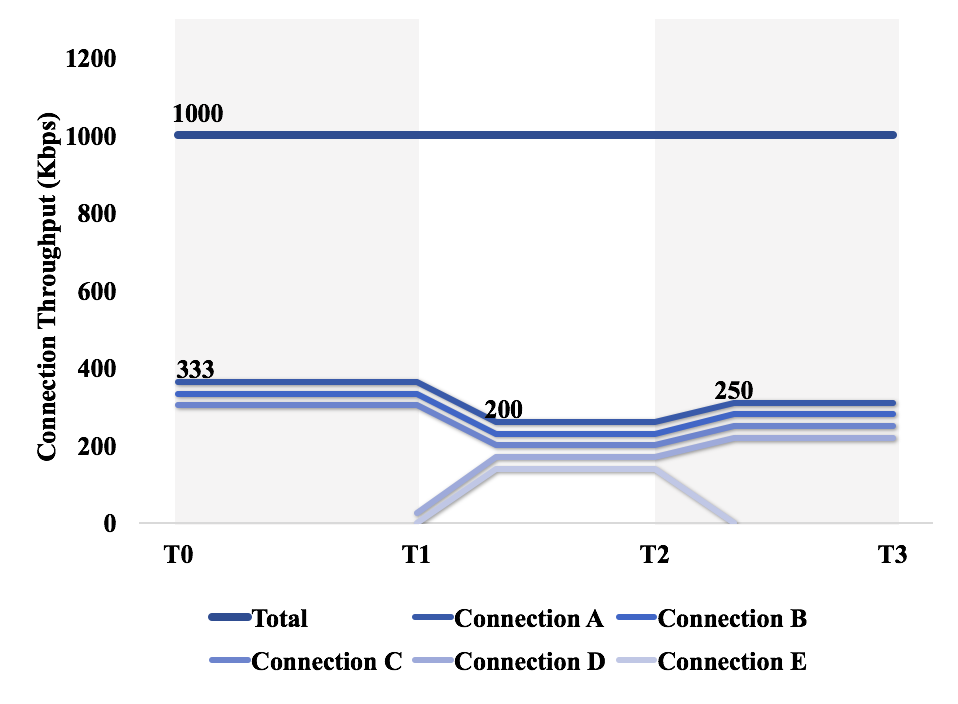
\includegraphics[width=0.8\textwidth]{./fig/mft_qos_rate_app}
\caption{Illustration of rate limiting for a certain application.}
\label{fig:mft_qos_rate_app}
\end{figure}

\subsubsection{The Flow Table Order of Forwarding and QoS Service}
Because the location of NAT, DHCP, and the firewall have been determined, we only need to decide the arrangement of QoS and forwarding. Assume that we place the QoS flow table after the forwarding flow table. In addition, we have only two services enabled, forwarding and QoS; therefore, the packet-in rule is in the last flow table of active service, Qos service. Then, suppose that a host is not limited by QoS policies. The first packet is not affected in both arrangements. For the subsequent packets, a difference can be observed. The packets that satisfy the rules in the forwarding flow table can not match rate limit rules in QoS flow table, because the host is not limited by QoS service; instead. As a result, the packets cause packet-in events by matching the packet-in rule in QoS service. This is unexpected because the packets already get the out-port action from the forwarding service. That is, it is not necessary to send these packet go to controller, and any packet-in event increases the controller’s load.

To reduce this load on the controller, we place the QoS flow table ahead of the forwarding flow table. In this scenario, all packets that pass through the QoS flow table continue to proceed to the forwarding flow table without satisfying any QoS rules. Then, all packets except the first packet are merely forwarded by the forwarding service instead of causing packet-in events. Thus, the controller’s load decreases.
